\section{Resultados obtenidos}
\subsection{Integración de las funciones en C para Interfaz}
Como se explicó anteriormente, el código utilizado para la creación de la interfaz gráfica, implementa varias funciones que son parte del correcto funcionamiento de la misma. Este permite la combinación de las funciones de GTK y del puerto serial para dar como resultado el control del vehículo de manera inalámbrica, por medio de un módulo \textit{bluetooth} que se puede conectar sin ningún problema con la computadora y así mismo con el código. Por esta razón, al correr el programa se obtiene como resultado la siguiente ventana que corresponde al control del Autonomous Vehicle for Tracking and Control Aplications (AuVeTA):
\begin{figure}[H]
    \centering
    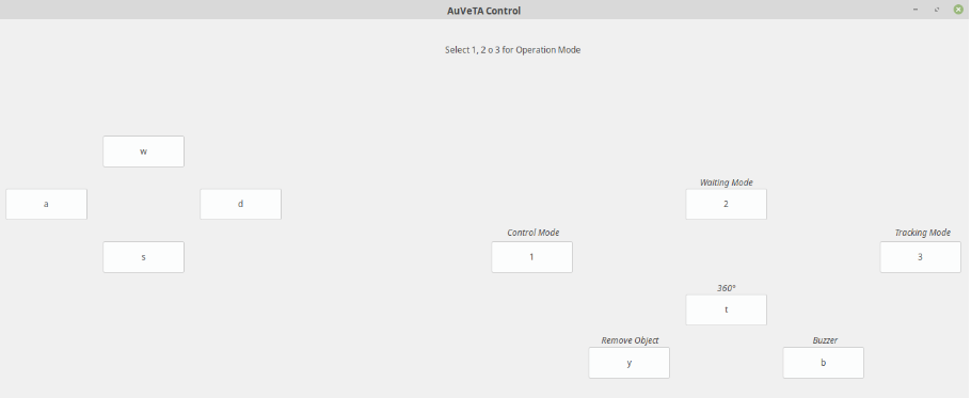
\includegraphics[width = 14cm]{imagenes/interfaz.png}
    \caption{Interfaz Gráfica (Autoría propia)}
    
\end{figure}

\subsection{Implementación del vehículo}
Tras la integración de todos los subsistemas para la conformación del vehículo y la realización de las pruebas correspondientes se produce a efectuar las pruebas críticas finales con el sistema completamente integrado, que implican tanto el funcionamiento del \textit{hardware} como el \textit{software} y las interacciones que existen entre ambos subsistemas. 

Como se ha abordado en la sección 3 de experimentos y pruebas, se obtienen resultados positivos para cada subsistema y además para la integración como un todo. El comportamiento de los sensores de obstáculo y de \textit{tracking} fue el esperado, ya que tanto la detección de objetos para su respectiva remoción como el sensor encargado de enviar la señal indicando el final de la pista y el que detecta la pista en el suelo funcionaron de manera correcta durante la demostración.

Cabe destacar que para la demostración se esperaba contar con una superficie de trabajo clara y regular, pero en el edificio en el que se realizó la demostración el suelo no reunía las condiciones de uniformidad de color necesarias para el funcionamiento del sensor de tracking, por tal motivo se optó por utilizar hojas blancas en el suelo y encima de ellas una cinta de color negro para garantizar el funcionamiento del sensor; ahora bien, este cambio afectó el rodamiento de las llantas y del tercer apoyo por el cambio en la aspereza de la superficie y por tanto además la cantidad de potencia que se utiliza en los motores para el movimiento en el \textit{\´´Tracking Mode"} del vehículo, por lo cual fue necesario realizar una modificación de última hora en el código; el aspecto de modificación de potencia de motores se tenia previsto por lo cual solo fue necesario ajustar una de las variables del código para lograr la modificación de manera rápida y sencilla de la cantidad de potencia enviada a los motores.